\documentclass{article} 

\def\rootdir{../}

\usepackage{graphicx}
\usepackage{times}
\usepackage{multicol}
\usepackage{multirow}
\usepackage{latexsym}
\usepackage{url}
\usepackage{xspace}
\usepackage{verbatim}
\usepackage{booktabs}
\usepackage{fullpage}
\usepackage{fancyvrb}
\usepackage{color}
\usepackage{listings}
\usepackage{amsthm}
\usepackage{amsmath}
\usepackage{enumerate}
\usepackage{subfigure}
\usepackage[sectionbib]{bibunits}
\usepackage{hyperref}
\usepackage{rotating}
\usepackage{Tabbing}
\usepackage[all]{xy}
\usepackage[textsize=scriptsize,textwidth=1cm]{todonotes}

\newlength{\tab}
\setlength{\tab}{1em}
\setlength{\parindent}{0pt}
\setlength{\parskip}{6pt}
\setlength{\evensidemargin}{0.0cm}
\setlength{\oddsidemargin}{0.0cm}
\setlength{\textwidth}{16cm}
%  \setlength{\headsep}{0cm}
\setlength{\headheight}{0cm}
\setlength{\topmargin}{0cm}
\setlength{\textheight}{23cm}
\setlength{\itemsep}{0pt}
\setlength{\topsep}{0pt}


\definecolor{javared}{rgb}{0.6,0,0} % for strings
\definecolor{javagreen}{rgb}{0.25,0.5,0.35} % comments
\definecolor{javapurple}{rgb}{0.5,0,0.35} % keywords
\definecolor{javadocblue}{rgb}{0.25,0.35,0.75} % javadoc
\definecolor{javabackground}{rgb}{0.9,0.9,0.9}
\definecolor{javablack}{rgb}{0,0,0}

\lstset{language=Ada,
  backgroundcolor=\color{javabackground},
  basicstyle=\ttfamily\fontsize{10}{12}\selectfont,
  keywordstyle=\color{javablack}\bfseries,
  aboveskip={1.5\baselineskip},
  stringstyle=\color{javared},
  commentstyle=\color{javagreen},
  morecomment=[s][\color{javadocblue}]{/**}{*/},
  numbers=left,
  numberstyle=\tiny\color{black},
  frame=single,
  numbersep=10pt,
  stepnumber=1,
  tabsize=8,
  xleftmargin=0ex,
  xrightmargin=0ex,
  showspaces=false,
  showstringspaces=false,
  aboveskip=0.5ex
}

\newtheoremstyle{defstyle} % name of the style to be used
  {\parskip} % measure of space to leave above the theorem. E.g.: 3pt
  {\parskip} % measure of space to leave below the theorem. E.g.: 3pt
  {}% name of font to use in the body of the theorem
  {}% measure of space to indent
  {\bf}% name of head font
  {\\}% punctuation between head and body
  {.5em}% space after theorem head; " " = normal interword space
  {\thmname{#1}\thmnumber{ #2}~~ {\rm \thmnote{(#3)}}}% header

\theoremstyle{defstyle}
\newtheorem{mydefinition}{Definition}[chapter]
\newenvironment{definition}{\begin{mydefinition}}{$\Box$\end{mydefinition}}

\newtheorem{myexample}{Example}[chapter]
\newenvironment{example}{\begin{myexample}}{$\Box$\end{myexample}}

\newtheorem{myexercise}{Exercise}[chapter]
\newenvironment{exercise}{\begin{myexercise}}{$\Box$\end{myexercise}}


\algnewcommand\algorithmicskip{\textbf{skip}}
\algnewcommand\algorithmicdone{\textbf{done}}
\algrenewcommand\algorithmicindent{2.0em}%


\def\all{\texttt{\textbf{all}}~}
\def\no{\texttt{\textbf{no}}~}
\def\some{\texttt{\textbf{some}}~}
\def\lone{\texttt{\textbf{lone}}~}
\def\one{\texttt{\textbf{one}}~}
\def\set{\texttt{\textbf{set}}~}
\def\alet{\texttt{\textbf{let}}~}


\begin{document}

%----------------------------------------------------------------------
%    Title Page
%

\tutorialtitle{3}

\section*{Introduction}

This workshop is about safety analysis. In particular we'll be using
HAZOPS (exploratory) to explore
the design of a Brake-by-Wire braking system. There are two main
brakes on a road vehicle:

\begin{description}

\item[The main service brake] --- This is the braking system that is
  typically operated by the foot pedal inside a car. It consists of
  the four rotors --- or discs --- in the wheels, calipers to slow or
  stop vehicle by slowing or stopping the rotors a foot hydraulic or
  electronic assisted actuation system for transferring the actions of
  the driver to the calipers.

  The major function of the service brake is to control the speed of
  the vehicle and to bring it to a complete stop when necessary.

  In emergencies the service brake must stop the vehicle in the
  shortest possible distance.

\item[The park brake] --- This is the brake used for holding the car
  in position while parked or while momentarily stopped. In current
  vehicles the park brake is operated by a lever in the middle of the
  vehicle next to the driver's position.

  The park brake has a number of functions:
  \begin{itemize}

  \item to hold the vehicle in place when parked and this includes
    parking on slopes and inclines and all types of surfaces, for
    example, road surfaces, wet road surfaces, slippery road surfaces,
    rocky surfaces or sand;

  \item to act as an emergency service brake; and 

  \item and for emergency turns. 

  \end{itemize}

\end{description}

Consider the design of a by-wire park brake in which the lever is
replaced by a button on the steering wheel, a computer controlled
system that detects wheel slip and locks the wheels in places, or if
the vehicle is rolling, engages the engine to hold the vehicle in
place.

The park brake works via a special motor that employs the rear
calipers to clamp the rear wheels and so stop the vehicle from
rolling.  If the car is rolling the park brake ECU interacts with the
motor --- if the motor is switched on --- and uses the motor to stop
the roll and keep the car in position. When the car is switched off a
rod is inserted via a small rear motor into the rear wheel rotors to
stop them from moving. For a schematic see Figure~\ref{fig:pb}.
\begin{figure}[htbp]
\centering
  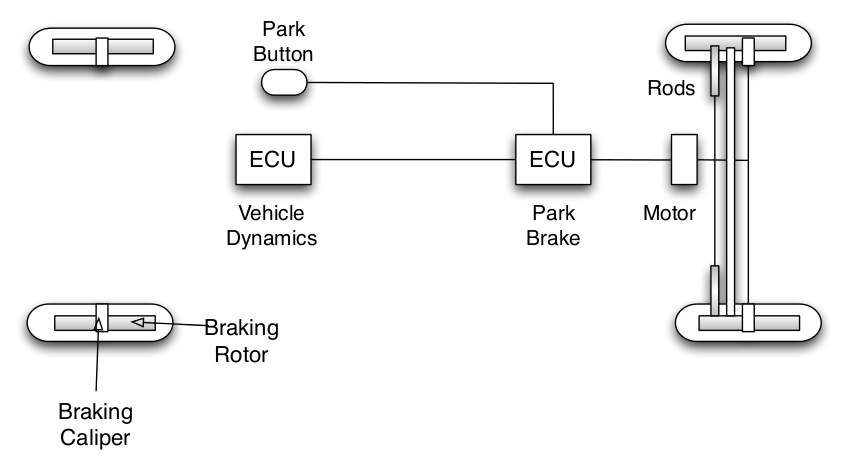
\includegraphics[width=0.80\textwidth]{./figs/ParkBrake}
  \caption{The design of the park brake system.}
  \label{fig:pb}
\end{figure}

The park brake ECU must therefore perform the following functions:
\begin{enumerate}
  \item Detect if the car's engine is switched on or not.
\item Engage the park brake when the button is pressed. 
\item Detect if the car is rolling when the park brake is on and
  employ the engine to compensate if the engine is switched on.
\end{enumerate}

\section*{Your tasks}

\begin{enumerate}

 \item Perform a hazard and operability study on the communications channels
in the design. The HAZOP guidewords are shown in Table~\ref{tab:hazop-guidewords}.

\begin{table}[!h]
\centering
\begin{tabular}{lp{11cm}}
 \toprule
      \textbf{Guide Word} & \textbf{Deviation}\\
 \midrule
      NO or NONE & This is the complete negation of the design intention. No
      part of the intention is achieved and nothing else happens.\\
      MORE & This is a quantitative increase.\\
      LESS & This is a quantitative decrease.\\
      AS WELL AS & All the design intention is achieved together with additions.\\
      PART OF & Only some of the design intention is achieved. \\
      REVERSE & The logical opposite of the intention is achieved.\\
      OTHER THAN & Complete substitution, where no part of the original
      intention is achieved but something quite different happens. \\
    EARLY  & Something happens earlier than expected relative to clock time.\\
    LATE & Something happens later than expected relative to clock time. \\
    BEFORE & Something happens before it is expected, relating to
    order or sequence.\\
    AFTER & Something happens after it is expected, relating to order or sequence.\\
\bottomrule
\end{tabular}
\caption{HAZOP guidewords}
\label{tab:hazop-guidewords}
\end{table}

 \item Perform a fault-tree analysis for the following hazard that can occur in a system for automatically administering insulin to a patient. The hazard to analyse is the case in which an incorrect dosage of insulin is delivered:

\begin{quote}
 Incorrect insulin dosage can be caused in three broad ways: an incorrect measure of the sugar level, incorrect delivery of dosage, or the dosage is delivered at the wrong time due to a timer failure. The sugar level is measured by a pair of sensors, and the resulting dosage is computed. The value from the first sensor is always used, unless no value is received from it (assumed to have failed), in which case the second sensor value is used.  The system must compute the insulin dosage and send the correct computation to the pump, which delivers the dosage.
Computation of sugar and insulin dosage can fail due to an incorrect algorithm or from arithmetic computations in the hardwarde.
\end{quote}

\begin{comment}
\item Perform a failure modes and effects analysis --- an FMEA. Your FMEA
should use a table with the headings below. A spreadsheet is available on the LMS and in the subject repository, which contains a template FMEA worksheet.

\begin{description}
\item[Item or Function] --- List the name of the item or the function
  that is being analysed in the row.
\item[Potential Failure Mode] --- List the potential failure
  modes. Failure modes are not specific instances of failure but
  rather types of failure associated with the component or item under
  investigation.
\item[Potential Effects of the Failure] --- Use the design to
  determine what such a failure will cause. Be careful of the chain of
  causal reasoning.
\item[Potential Causes] --- Hypothesise potential causes of the
  failure.
\item[Severity (Rating)] --- Estimate the severity of the failure mode
  using Table~\ref{tab:severity}.
\item[Occurrence (Rating)] Estimate the frequency of the failure mode
  using Table~\ref{tab:occurrences}.
\item[Current Controls] --- List any existing ways in the design that
  the failure mode is controlled or mitigated.
\item[Recommended Actions] --- If there any actions that can reduce or
  mitigate the effects of the failure mode then list these here.
\item[New Severity] --- Estimate the new severity rating if the
  recommended actions are followed.  
\item[New Occurrence] --- Estimate the new occurrence rating if the
  recommended actions are followed.  	
\end{description}

\end{enumerate}

\begin{table}[!h]
\centering
\begin{tabular}{lp{11cm}}
  \toprule
  {\bf Rating}  & {\bf Meaning} \\
  \midrule
  {\bf 1} & No known occurrences on similar products or processes\\
  {\bf 2} & Low (relatively few failures)\\
  {\bf 3} &	Moderate (occasional failures)\\
  {\bf 4} & High (repeated failures)\\
  {\bf 5} & Very high (failure is almost inevitable)\\
  \bottomrule
\end{tabular}
\caption{Occurrence Ratings Tables}
\label{tab:occurrences}
\end{table} 

\begin{table}[!h]
\centering
\begin{tabular}{lp{11cm}}
  \toprule
  {\bf Rating}  & {\bf Meaning} \\
  \midrule
  {\bf 1} & No effect\\
  {\bf 2} & Very minor (only noticed by discriminating customers)\\
  {\bf 3} & Minor (affects very little of the system, noticed by average
  customer) \\
  {\bf 4} &Moderate (most customers are annoyed)\\
  {\bf 5} & High (causes a loss of primary function; customers
  are dissatisfied)\\
  {\bf 6} & Very high and hazardous (product becomes
  inoperative; customers angered; the failure may result unsafe
  operation and possible injury)\\
  \bottomrule
\end{tabular}
\caption{Severity Ratings Tables}
\label{tab:severity}
\end{table} 
\end{comment}

\end{enumerate}

\end{document}

% LocalWords:  HAZOPS FMEA calipers HAZOP guidewords lp
